\section{区间表示法}

\begin{definition}[区间]
    另一种表示 一个范围内的所有实数构成的数集 的方法是 区间．其形如：
    \begin{multicols}{2}
        \begin{enumerate}
            \item $[a, b]=\{x \in \mathbb{R} \mid a \leq x \leq b\}$ ．
            \item $[a, b)=\{x \in \mathbb{R} \mid a \leq x<b\}$ ．
            \item $(a, b]=\{x \in \mathbb{R} \mid a<x \leq b\}$ ．
            \item $(a, b)=\{x \in \mathbb{R} \mid a<x<b\}$ ．
            \item $[a,+\infty)=\{x \in \mathbb{R} \mid x \geq a\}$ ．
            \item $(a,+\infty)=\{x \in \mathbb{R} \mid x>a\}$ ．
            \item $(-\infty, b]=\{x \in \mathbb{R} \mid x \leq b\}$ ．
            \item $(-\infty, b)=\{x \in \mathbb{R} \mid x<b\}$ ．
            \item $(-\infty,+\infty)=\mathbb{R}$ ．
        \end{enumerate}
    \end{multicols}

    总之，我们用方括号表示包含端点，圆括号表示不包含端点．正、负无穷一般用圆括号．
    两端包含端点的称为 闭区间，两端不包含端点的称为 开区间，一端包含一端不包含的称为 半开半闭区间．
    另外，用区间的并表示「或」，如：
    $$(-\infty, 1) \cup\left[\frac{3}{2},+\infty\right)=\left\{x \in \mathbb{R} \mid x<1\right. \text{或} \left.x \geq \frac{3}{2}\right\}, ~(-\infty, 2) \cup (2,+\infty)=\{x \in \mathbb{R} \mid x \neq 2\}$$
    \begin{tips}
        正无穷 $+\infty$ 中的正号 + 有时会被省略，但有时只用 $\infty$ 又表示 $\pm \infty$ ．具体意义须结合上下文理解．
    \end{tips}
\end{definition}

\subsection{开区间与闭区间}

\begin{definition}[区间的类型]
    根据端点的包含情况，区间可以分为以下几种类型：

    \begin{multicols}{2}
        \textbf{开区间}是指两端都不包含端点的区间，记作 $(a, b)$ ．
        \begin{center}
            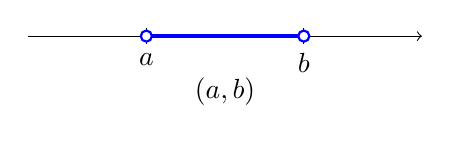
\begin{tikzpicture}
                \draw[->] (-0.5,0) -- (4.5,0);
                \foreach \x/\label in {1/a, 3/b}
                \draw (\x,0.1) -- (\x,-0.1) node[below] {$\label$};
                \draw[very thick, blue] (1,0) -- (3,0);
                \draw[blue, fill=white, thick] (1,0) circle (2pt);
                \draw[blue, fill=white, thick] (3,0) circle (2pt);
                \node at (2,-0.7) {$(a,b)$};
            \end{tikzpicture}
        \end{center}

        \columnbreak

        \textbf{闭区间}是指两端都包含端点的区间，记作 $[a, b]$ ．
        \begin{center}
            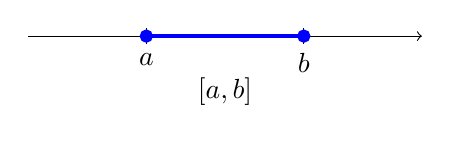
\begin{tikzpicture}
                \draw[->] (-0.5,0) -- (4.5,0);
                \foreach \x/\label in {1/a, 3/b}
                \draw (\x,0.1) -- (\x,-0.1) node[below] {$\label$};
                \draw[very thick, blue] (1,0) -- (3,0);
                \filldraw[blue, thick] (1,0) circle (2pt);
                \filldraw[blue, thick] (3,0) circle (2pt);
                \node at (2,-0.7) {$[a,b]$};
            \end{tikzpicture}
        \end{center}
    \end{multicols}

    \textbf{半开半闭区间}是指一端包含端点而另一端不包含端点的区间，记作 $[a, b)$ 或 $(a, b]$ ．
    \begin{center}
        % --- 这是修正错误的重点区域 ---
        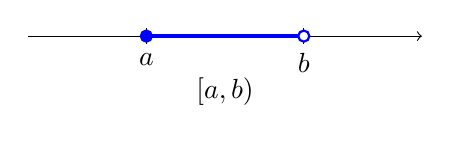
\begin{tikzpicture}
            \draw[->] (-0.5,0) -- (4.5,0);
            \foreach \x/\label in {1/a, 3/b}
            \draw (\x,0.1) -- (\x,-0.1) node[below] {$\label$}; % <-- 添加了分号
            \draw[very thick, blue] (1,0) -- (3,0);
            \filldraw[blue, thick] (1,0) circle (2pt);      % a点是实心
            \draw[blue, fill=white, thick] (3,0) circle (2pt); % b点是空心
            \node at (2,-0.7) {$[a,b)$};
        \end{tikzpicture}
        \hspace{1cm}
        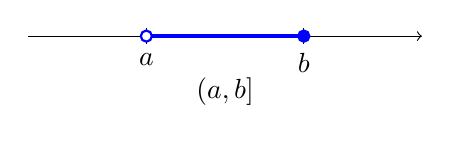
\begin{tikzpicture}
            \draw[->] (-0.5,0) -- (4.5,0);
            \foreach \x/\label in {1/a, 3/b}
            \draw (\x,0.1) -- (\x,-0.1) node[below] {$\label$}; % <-- 添加了分号
            \draw[very thick, blue] (1,0) -- (3,0);
            \draw[blue, fill=white, thick] (1,0) circle (2pt); % a点是空心
            \filldraw[blue, thick] (3,0) circle (2pt);      % b点是实心
            \node at (2,-0.7) {$(a,b]$};
        \end{tikzpicture}
    \end{center}
\end{definition}


\begin{exercise}
    画出以下区间的示意图，并标出端点：
    \begin{multicols}{2}
        \begin{enumerate}
            \item $[1, 2)$
            \item $(2, 3]$
                  \columnbreak
            \item $(-\infty, 0]$
            \item $[0, +\infty)$
        \end{enumerate}
    \end{multicols}
\end{exercise}

\begin{problem}
用区间表示下列不等式的解集．
\begin{multicols}{2}
    \begin{enumerate}
        \item $\{x \mid 2 \leq x \leq 3\}$
        \item $\{x \mid 4<x<6\}$
              \columnbreak
        \item $\{x \mid 1 \leq x<2\}$
        \item $\{x \mid 7<x \leq 9\}$
    \end{enumerate}
\end{multicols}
\end{problem}

\subsection{无穷区间}

\begin{definition}[无穷区间]
    无穷区间是指包含正无穷或负无穷的区间，记作 $(-\infty, a)$、$(-\infty, a]$、$[a, +\infty)$ 或 $(a, +\infty)$ ．
    \begin{center}
        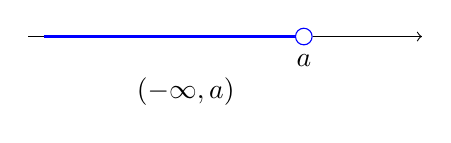
\begin{tikzpicture}
            \draw[->] (-0.5,0) -- (4.5,0);
            \foreach \x/\label in {3/a}
            \draw (\x,0.1) -- (\x,-0.1) node[below] {$\label$};
            \draw[very thick, blue] (-0.3,0) -- (3,0);
            \filldraw[white] (3,0) circle (3pt);
            \draw[blue] (3,0) circle (3pt);
            \node at (1.5,-0.7) {$(-\infty,a)$};
        \end{tikzpicture}
        \hspace{1cm}
        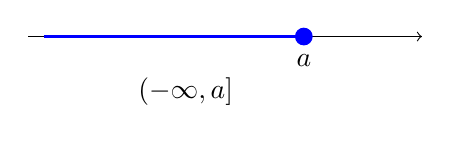
\begin{tikzpicture}
            \draw[->] (-0.5,0) -- (4.5,0);
            \foreach \x/\label in {3/a}
            \draw (\x,0.1) -- (\x,-0.1) node[below] {$\label$};
            \draw[very thick, blue] (-0.3,0) -- (3,0);
            \filldraw[blue] (3,0) circle (3pt);
            \node at (1.5,-0.7) {$(-\infty,a]$};
        \end{tikzpicture}

        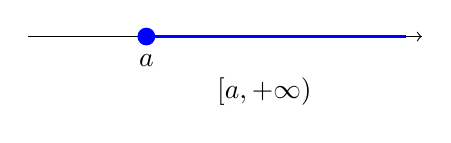
\begin{tikzpicture}
            \draw[->] (-0.5,0) -- (4.5,0);
            \foreach \x/\label in {1/a}
            \draw (\x,0.1) -- (\x,-0.1) node[below] {$\label$};
            \draw[very thick, blue] (1,0) -- (4.3,0);
            \filldraw[blue] (1,0) circle (3pt);
            \node at (2.5,-0.7) {$[a,+\infty)$};
        \end{tikzpicture}
        \hspace{1cm}
        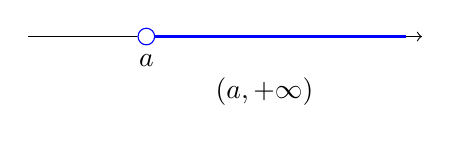
\begin{tikzpicture}
            \draw[->] (-0.5,0) -- (4.5,0);
            \foreach \x/\label in {1/a}
            \draw (\x,0.1) -- (\x,-0.1) node[below] {$\label$};
            \draw[very thick, blue] (1,0) -- (4.3,0);
            \filldraw[white] (1,0) circle (3pt);
            \draw[blue] (1,0) circle (3pt);
            \node at (2.5,-0.7) {$(a,+\infty)$};
        \end{tikzpicture}
    \end{center}
\end{definition}

\begin{example}
    （2014·陕西文科·1）已知集合 $M=\{x \mid x \geq 0\}, N=\left\{x \mid x^2<1, x \in R\right\}$ ，则 $M \cap N=$ （\qquad）
    \begin{tasks}(4)
        \task $[0,1]$
        \task $(0,1)$
        \task $(0,1]$
        \task $[0,1)$
    \end{tasks}
\end{example}

\v{4em}

\begin{example}
    （2014·山东文·2）设集合 $A=\left\{x \mid x^2-2 x<0\right\}, B=\{x \mid 1 \leq x \leq 4\}$ ，则 $A \cap B=$ （\qquad）
    \begin{tasks}(4)
        \task $(0,2]$
        \task $(1,2)$
        \task $[1,2)$
        \task $(1,4)$
    \end{tasks}
\end{example}

\v{4em}

\begin{example}
    （2014·辽宁文·1）已知全集 $U=R, A=\{x \mid x \leq 0\}, B=\{x \mid x \geq 1\}$ ，则集合 $\mathrm{C}_U(A \cup B)=$ \underline{\qquad}.
\end{example}

\v{4em}

\begin{example}
    （2015·浙江文·1）已知集合 $\mathrm{P}=\left\{x \mid x^2-2 x \geq 3\right\}, \mathrm{Q}=\{x \mid 2<x<4\}$ ，则 $\mathrm{P} \cap \mathrm{Q}=$ （\qquad）
    \begin{tasks}(4)
        \task $[3,4)$
                        \task $(2,3]$
        \task $(-1,2)$
        \task $(-1,3]$
    \end{tasks}
\end{example}

\v{4em}

\begin{example}
    （2015·II文·1）已知集合 $A=\{x \mid-1<x<2\}, B=\{x \mid 0<x<3\}$ ，则 $A \cup B=$ （\qquad）
    \begin{tasks}(4)
        \task $(-1,3)$
        \task $(-1,0)$
        \task $(0,2)$
        \task $(2,3)$
    \end{tasks}
\end{example}

\v{4em}

